\documentclass[12pt]{standalone}
\usepackage[english]{babel}
\usepackage[utf8]{inputenc}

\usepackage{comment}
\usepackage{amsmath}
\usepackage{tikz}
\usepackage{circuitikz} % for circuits!
\usetikzlibrary{arrows.meta} % for loads
\usepackage{float}
\usetikzlibrary{positioning}

\begin{document}
	
	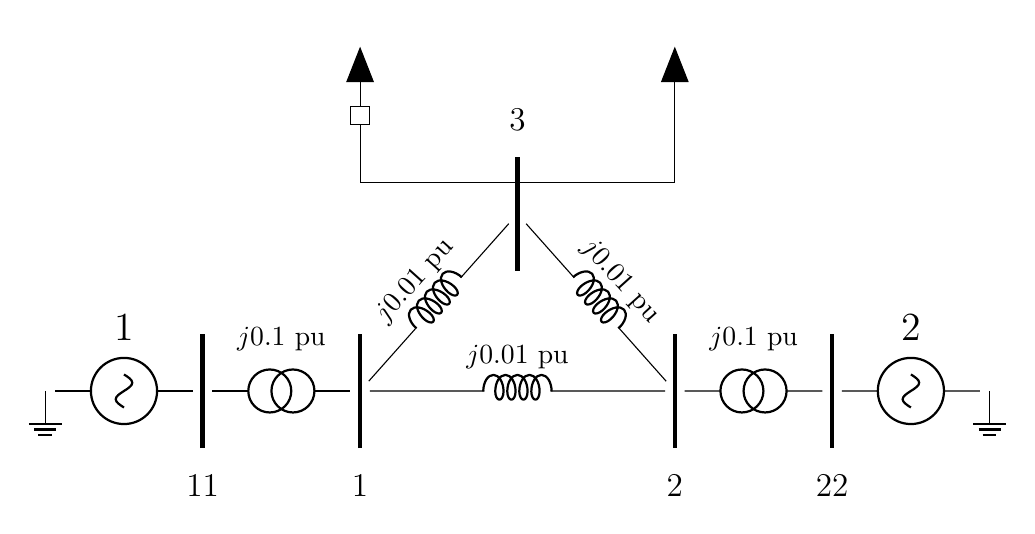
\begin{tikzpicture} [american voltages,scale=.8, 
		breaker/.style={rectangle,draw=black,fill=white},
		load/.style={-{Triangle[length=4.5mm,width=3.5mm,open,fill=black]}},
		node distance = 2 cm and 1.75cm]
		
		% node positions
		\node (start) at (0,0) {};
		\node[right = of start](bus11) {};
		\node[right = of bus11](bus1) {};
		\node[above right = of bus1](bus3) {};
		\node[below right = of bus3](bus2) {};
		\node[right = of bus2](bus22) {};
		\node[right = of bus22](end) {};
		\node[above right = of bus3](load1){};
		\node[above left = of bus3](load2){};
		
		%draw buses
		\foreach \name in {1,11,22,2,3}
		\draw[ultra thick] ([yshift=-0.75cm]bus\name.south) -- ([yshift=+0.75cm]bus\name.north);
		
		% gen
		\draw (start) node[ground]{} to [sV, n=G1] (bus11)  {};
		\draw (end) node[ground]{} to [sV, n=G2] (bus22)  {};
		\foreach \name in{1, 2}
		\draw (G\name)++(0,1) node (G\name){\Large \name};
		
		% xfmr
		\draw (bus11) to [voosource, l=$j0.1$ pu]  (bus1) {};
		\draw (bus2) to [voosource, l=$j0.1$ pu]  (bus22) {};
		
		% lines
		\draw (bus1) to [L, l=$j0.01$ pu] (bus2); 
		\draw (bus1) to [L, l=$j0.01$ pu] (bus3); 
		\draw (bus3) to [L, l=$j0.01$ pu] (bus2); 
		
		% load
		\draw[load] (bus3.center)++(0,.5) -| (load1) ;
		\draw[load] (bus3.center)++(0,.5) -| (load2) ;
		\draw (load2)++(0,-1.25) node[breaker] {};
		
		%bus labels below
		\foreach \name in {1,11,22,2}
		\draw (bus\name) ++(0,-1.5) node {\large{\name}};
		%bus labels above
		\foreach \name in {3}
		\draw (bus\name) ++(0,+1.5) node {\large{\name}};
		
	\end{tikzpicture}
\begin{comment}	
	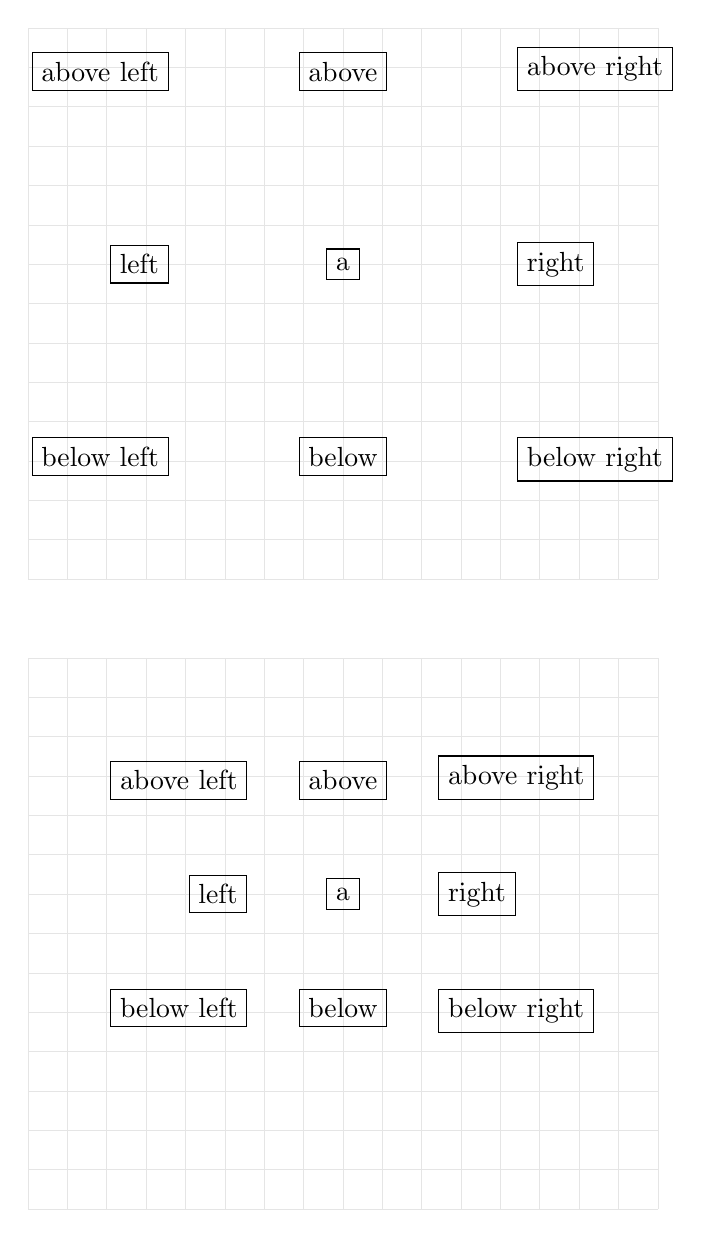
\begin{tikzpicture} 
	\draw[help lines,step=5mm,gray!20] (-4,-4) grid (4,3);
	\node[draw] (a) at (0,0) {a};  
	\foreach \pos in {above,above right,right,below right,below,below left,left,above left}
	\node[draw,\pos = of a] () {\pos};
	
	\begin{scope}[yshift=8cm,node distance=2cm and 2cm]
	\draw[help lines,step=5mm,gray!20] (-4,-4) grid (4,3);
	
	\node[draw] (a) at (0,0) {a};  
	\foreach \pos in {above,above right,right,below right,below,below left,left,above left}
	\node[draw,\pos = of a] () {\pos};
	\end{scope}
	\end{tikzpicture} 
	
\end{document}


\begin{document}

%3 gen 8 bus
\begin{figure}[H]% system diagram
	\begin{center} 
		% 4 bus, infinite gen power system
		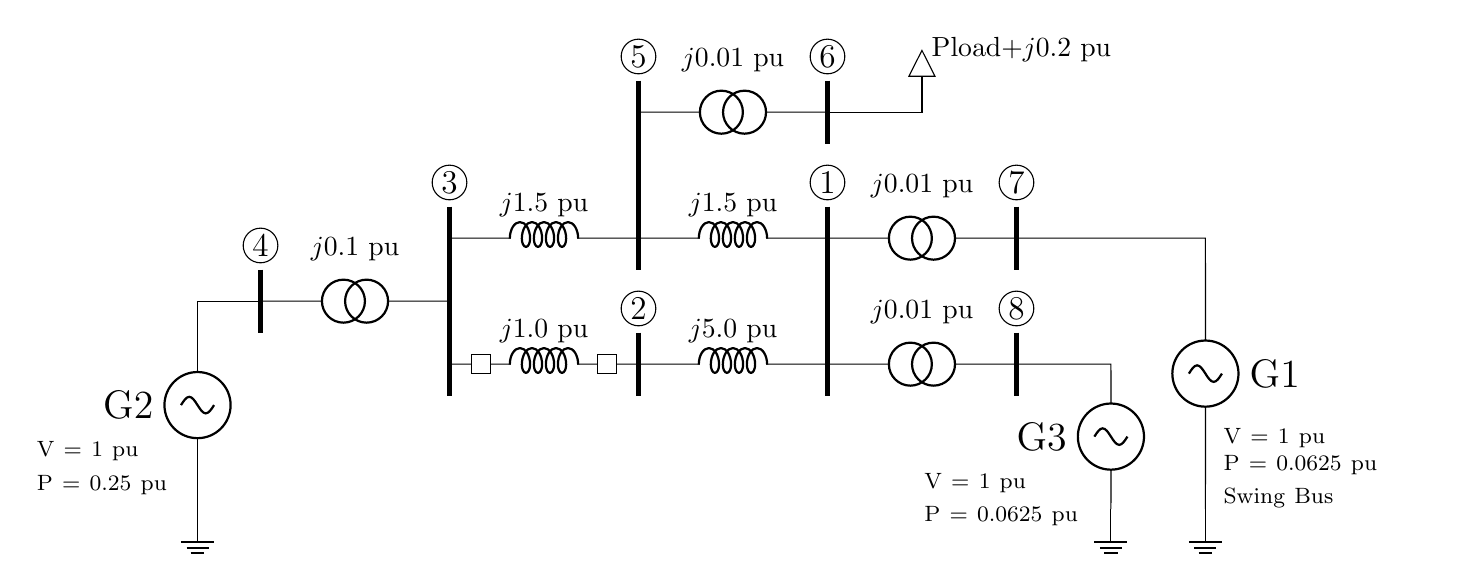
\begin{tikzpicture} [american voltages,scale=.8, 
		breaker/.style={rectangle,draw=black,fill=white}]
		
		% Generators 
		\draw (1,2) to (0,2) to [sV, n=G2] (0,-1.3) node[ground] {}; % G2
		\draw (13,3) to (16,3) to [sV, n=G1] (16,-1.3) node[ground] {}; % g1
		\draw (13,1) to (14.5,1) to [sV, n=G3] (14.5,-1.3) node[ground] {}; % g3
		
		% Labels for gens
		\draw (G2) ++(-1.1,0) node (G2L){\Large G2};
		\draw (G2L) ++(-0.2,-1) node[text width=2cm] {\footnotesize V = 1 pu\\ P = 0.25 pu};
		\draw (G1) ++(1.1,0) node (G1L){\Large G1};
		\draw (G1L) ++(+0.75,-1.5) node[text width=2.5cm] {\footnotesize V = 1 pu\\ P = 0.0625 pu\\Swing Bus};
		\draw (G3) ++(-1.1,0) node (G3L){\Large G3};
		\draw (G3L) ++(-.3,-1) node[text width=2.5cm] {\footnotesize V = 1 pu\\P = 0.0625 pu};
		
		% inductances
		\draw (1,2) to [voosource, l=$j0.1$ pu]  (4,2) {}; % g2 xfmr X
		\draw (4,3) to [L, l=$j1.5$ pu] (7,3); %top branch
		\draw (7,3) to [L, l=$j1.5$ pu] (10,3); %top branch
		\draw (4,1) to [L, l=$j1.0$ pu] (7,1); %lower branch left
		\draw (7,1) to [L, l=$j5.0$ pu] (10,1); %lower branch right
		\draw (7,5) to [voosource, l=$j0.01$ pu] (10,5); %add branch right
		\draw (10,1) to [voosource, l=$j0.01$ pu] (13,1); %xfm to G3
		\draw (10,3) to [voosource, l=$j0.01$ pu] (13,3); %xfm to G1
		
		% Draw Busses - named nodes at top of line
		\draw [ultra thick] (1, 2.5) node (bus4) {} -- (1,1.5) ;	%bus 4
		\draw [ultra thick] (4, 3.5) node (bus3) {} -- (4,.5) ;		%bus 3
		\draw [ultra thick] (7, 1.5) node (bus2) {} -- (7,0.5);	%bus 2
		\draw [ultra thick] (7, 5.5) node (bus5) {} -- (7,2.5);		%bus 5
		\draw [ultra thick] (10, 3.5) node (bus1) {} -- (10,.5) ;	%bus 1
		\draw [ultra thick] (10, 5.5) node (bus6) {} -- (10,4.5) ;	%bus 6
		\draw [ultra thick] (13, 1.5) node (bus8) {} -- (13,0.5) ;	%bus 8
		\draw [ultra thick] (13, 3.5) node (bus7) {} -- (13,2.5) ;	%bus 7
		
		% Labels for busses
		\draw (bus1) ++(0,.1) node[anchor = south,circle,inner sep=1pt,draw] {\large{1}};
		\draw (bus2) ++(0,.1) node[anchor = south,circle,inner sep=1pt,draw] {\large{2}};
		\draw (bus3) ++(0,.1) node[anchor = south,circle,inner sep=1pt,draw] {\large{3}};
		\draw (bus4) ++(0,.1) node[anchor = south,circle,inner sep=1pt,draw] {\large{4}};
		\draw (bus5) ++(0,.1) node[anchor = south,circle,inner sep=1pt,draw] {\large{5}}; 
		\draw (bus6) ++(0,.1) node[anchor = south,circle,inner sep=1pt,draw] {\large{6}};
		\draw (bus7) ++(0,.1) node[anchor = south,circle,inner sep=1pt,draw] {\large{7}};
		\draw (bus8) ++(0,.1) node[anchor = south,circle,inner sep=1pt,draw] {\large{8}};
		% fault location
		%\draw (5.5,0.9) node {\textcolor{m}{\Huge \Lightning}};
		
		% Breakers
		%	\draw (7.5, 5) node [breaker] {};
		%	\draw (9.5, 5) node [breaker] {};
		%	\draw (10.5, 1) node [breaker] {};
		%	\draw (12.5, 1) node [breaker] {};
		\draw (4.5, 1) node [breaker] {};
		\draw (6.5, 1) node [breaker] {};
		
		% loads
		\draw[-{Triangle[length=3.5mm,width=3.5mm,open]}] (10,5)--(11.5,5)--(11.5,6) node[anchor = west] {Pload$+j0.2$ pu};
		%	\draw[-{Triangle[length=3.5mm,width=3.5mm,open]}] (7,-0.5)--(5.5,-0.5)--(5.5,-1.5) node[anchor = east] {$0.325+j0.15$ pu};
		\end{tikzpicture}
		\vspace{-1.5em}
		\caption{100 MVA Power system with generator powers for heavy Pload cases.}
		\label{p_sys}
	\end{center}
\end{figure}

\end{comment}


\end{document}